% Copyright (c) 2016 General Electric Company.  All rights reserved.
\documentclass[10pt]{article}

\usepackage{graphicx}
\usepackage{amssymb}
\usepackage{amsmath}
\usepackage{tikz}
\usepackage{algorithm2e}

\title{Csorba-Kurzer (CK) Similarity \\ \large US Patent 9,269,028}
\date{\today}
\author{Brett Csorba \and Jacob Kurzer}

\parindent 0px
\parskip 0pt

\newcommand{\bigO}[1]{\ensuremath{\operatorname{O}\left(#1\right)}}

\begin{document}
\maketitle

\section{Overview}
While numeric data is easy to compare and correlate, the same cannot be said for character strings.  What determines how similar \textit{cat} is to \textit{bat} and how similar both are to \textit{chat}?  The traditional approach used to determine this similarity can be defined by the edit distance or the number of character insertions, deletions, and transpositions to transform one character string to another.  This edit distance is also known as Damerau--Levenshtein distance.  While this metric produces accurate and useful measures of similarity, algorithms traditionally used to compute this distance have a \bigO{mn} running time, where m and n are the length of the input strings.  Faster running algorithms do exist that run in linear time, but these algorithms are limited by aspects such as machine word size or limit the range of the input strings they can operate on.\\[2ex]
Our algorithm calculates string similarity resulting in orders that strongly approximate traditional edit distance calculations while running in linear \bigO{m+n} time.  This is achieved through linear preprocessing steps of input strings that can be memoized for future string comparisons and linear character comparison steps.  Our approach is general purpose and has been shown to be effective in computing similarity of a variety of string types including machine produced hashed strings.  Applications range from finding patterns in phishing emails, evaluating network topology, and determining attack patterns on large scale data encompassing tens of thousands of string of variable lengths and hierarchies.\\[2ex]
Our algorithm will return a floating point value in the range of [0 1], 0 indicating perfect similarity and 1 indicating maximum dissimilarity.  A notable point is that we believe that this algorithm returns values which will satisfy the triangle inequality, allowing for pruning approaches when dealing with large data sets.  A Java implementation of this code is currently being used for server side computations.  The original implementation of the algorithm was in JavaScript, allowing this code to be highly portable and run client side on web applications, having the potential to reduce server computation time and costs.
  
  \section{Preprocess Strings}
  Our algorithm will first preprocess each of the input strings into a data structure which will allow the algorithm to find indexes of characters within each string.  These structures can be memorized in a hashtable structure preventing this step from being repeated for future comparisons against the input strings.\\[2ex]
  Each input string $s$ contains the character set $C$.  Create a hashtable $h$ for this string.  For each character $s_i$ in $s$, append the index $i$ of $s_i$ to the end of the List $l$ at key $s_i$.  As $i$ is always increasing, $l$ will be in sorted order.  Assuming \bigO{1} insertions, accesses, and edits for $h$ and \bigO{1} inserts into $l$, a string of length $m$ can be preprocessed in \bigO{m} time.
  
  \section{Comparing Strings}
  Preprocess strings $A$ and $B$ with lengths $m$ and $n$ into hashes $a$ and $b$ taking \bigO{m+n} time.  These strings are compared through both a measurement of dissimilarity in the character sets $C_a$ and $C_b$ and the different indexes of intersecting characters in these sets.  Three measures are kept track of, character similarity in string A ($S_A$), character similarity in string B, ($S_B$), and total disordering ($D$).\\[2ex]
  \begin{figure}[h]
    \centering
    \minipage{.5\textwidth}
    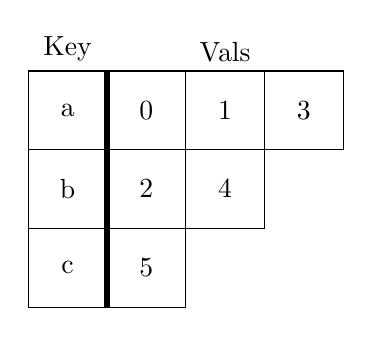
\begin{tikzpicture}
      \draw (.5,3) node[above] {Key};
      \draw (2.5,3) node[above] {Vals};
      \foreach \x in {0,...,4}
      \draw (\x,2) rectangle(3,3);
      \foreach \x in {0,...,3}
      \draw (\x,1) rectangle(2,2);
      \foreach \x in {0,...,2}
      \draw (\x,0) rectangle (1,1);
      \draw[line width=2pt] (1,3) to (1,0);
      \def\a{{"a",0,1,3}}
      \def\b{{"b",2,4}}
      \def\c{{"c",5}}
      \foreach \x in {0,...,3}
      \draw (.5+\x,2.5) node {\pgfmathparse{\a[\x]}\pgfmathresult};
      \foreach \x in {0,...,2}
      \draw (.5+\x,1.5) node {\pgfmathparse{\b[\x]}\pgfmathresult};
      \foreach \x in {0,...,1}
      \draw (.5+\x,.5) node {\pgfmathparse{\c[\x]}\pgfmathresult};
    \end{tikzpicture}
    \centering
    \caption{Hash for string $A=\text{aababc}$}
    \endminipage
    \centering
    \minipage{.5\textwidth}
    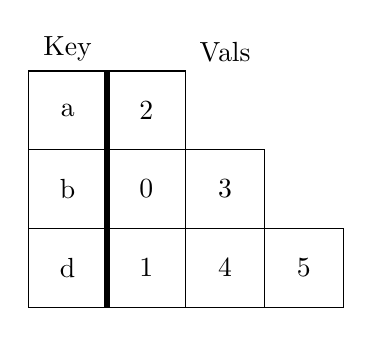
\begin{tikzpicture}
      \draw (.5,3) node[above] {Key};
      \draw (2.5,3) node[above] {Vals};
      \foreach \x in {0,...,2}
      \draw (\x,2) rectangle(2,3);
      \foreach \x in {0,...,3}
      \draw (\x,1) rectangle(2,2);
      \foreach \x in {0,...,4}
      \draw (\x,0) rectangle (1,1);
      \draw[line width=2pt] (1,3) to (1,0);
      \def\a{{"a",2}}
      \def\b{{"b",0,3}}
      \def\d{{"d",1,4,5}}
      \foreach \x in {0,...,1}
      \draw (.5+\x,2.5) node {\pgfmathparse{\a[\x]}\pgfmathresult};
      \foreach \x in {0,...,2}
      \draw (.5+\x,1.5) node {\pgfmathparse{\b[\x]}\pgfmathresult};
      \foreach \x in {0,...,3}
      \draw (.5+\x,.5) node {\pgfmathparse{\d[\x]}\pgfmathresult};
    \end{tikzpicture}
    \centering
    \caption{Hash for string $B=\text{bdabdd}$}
    \endminipage
  \end{figure}
  First, each key $k_a$ in $a$ is evaluated.  \\[2ex]
  If $k_a \notin b$, then add 1 to $S_A$.  \\[2ex]
  If $k_a \in b$, we need to compute how disordered the indexes of $l_{k_a}$ are compared to $l_{k_b}$.  Compare the lengths of $l_{k_a}$ and $l_{k_b}$.  Assign the shorter list to $c$ and the longer list to $d$.  Remember $c$ and $d$ are ordered.  
  \begin{figure}[h]
    \centering
    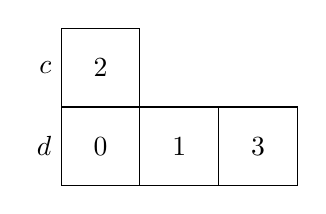
\begin{tikzpicture}
      \def\d{{0,1,3}};
      \draw (0,1) rectangle (1,2);
      \draw (0,1.5) node[left] {$c$};
      \draw (.5,1.5) node {2};
      \foreach \x in {0,...,2}{
      \draw (\x,0) rectangle (3,1);
      \draw (.5+\x,.5) node {\pgfmathparse{\d[\x]}\pgfmathresult};
      }
      \draw (0,.5) node[left] {$d$};
    \end{tikzpicture}
    \centering
    \caption{For $k_a=\text{a}$}
  \end{figure}\\[2ex]
For each index $c_i$ in $c$, find the first element in $d$ that is greater than $c_i$ by iterating through $d$.  For each element in $d$ that is less than or equal to $c_i$, push this element onto a stack $s$.\\[2ex]
\begin{figure}
  \centering
  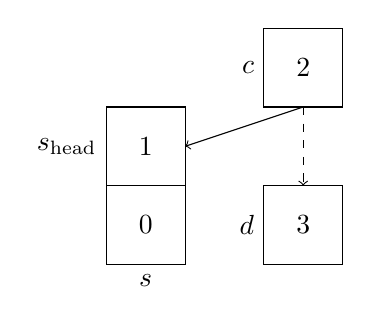
\begin{tikzpicture}
    \draw (0,0) rectangle (1,1);
    \draw (0,1) rectangle (1,2);
    \draw (.5,0) node[below] {$s$};
    \draw (0,1.5) node[left] {$s_{\text{head}}$};
    \draw (.5,.5) node {0};
    \draw (.5,1.5) node{1};

    \draw (2,2) rectangle (3,3);
    \draw (2,2.5) node[left] {$c$};
    \draw (2.5,2.5) node {2};

    \draw (2,0) rectangle (3,1);
    \draw (2,.5) node[left] {$d$};
    \draw (2.5,.5) node {3};

    \draw[->] (2.5,2) -- (1,1.5);
    \draw[dashed, ->] (2.5,2) -- (2.5,1);
  \end{tikzpicture}
  \caption{State after alignment, $k_a=\text{a}$}
\end{figure}

  If the total number of remaining indexes in $c$ and $d$ are equal and the stack is empty, this means that the smallest possible disordering would be to pair $c_1\rightarrow d_1, c_2\rightarrow d_2, ..., c_n\rightarrow d_n$.  Add to $D$ the absolute value of $c_1-d_1,c_2-d_2, ..., c_n – d_n$. There are no more letters then in $c$ to process.\\[2ex]
  \begin{figure}
    \centering
    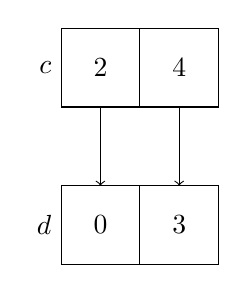
\begin{tikzpicture}
      \foreach \x in {0,...,2}
      \draw (\x,2) rectangle(2,3);
      \def\c{{2,4}}
      \foreach \x in {0,...,1}
      \draw (.5+\x,2.5) node {\pgfmathparse{\c[\x]}\pgfmathresult};
      \draw (0,2.5) node[left] {$c$};

      \foreach \x in {0,...,2}
      \draw (\x,0) rectangle(2,1);
      \def\d{{0,3}}
      \foreach \x in {0,...,1}
      \draw (.5+\x,.5) node {\pgfmathparse{\d[\x]}\pgfmathresult};
      \draw (0,.5) node[left] {$d$};

      \draw[->] (.5,2) -- (.5,1);
      \draw[->] (1.5,2) -- (1.5,1);
    \end{tikzpicture}
    \caption{State after alignment, $k_b=\text{b}$}
    
  \end{figure}
  If not, compare $d_j-c_i$ to $c_i-s_{\text{head}}$.  The smaller value is the index that is the closest to $c_i$.  Add this value to $D$.  If this is $d_j-c_i$, remove $d_j$ from $d$ so it is no longer evaluated.  If this is $c_i-s_{\text{head}}$, pop $s_{\text{head}}$ from $s$.  Continue to process the remaining $c_i$ in $c$ in this way.\\[2ex]
  After all remaining $c_i$ have been processed, $d$ and $s$ may contain still contain indexes.  If $d$ was assigned from $a$, add 1 to $S_A$ for each letter remaining in $d$ and in $s$.    If $d$ was assigned from $b$, add 1 to $S_B$ for each letter remaining in $d$ and in $s$.\\[2ex]\input{../projects/maven/now}

  Add the count of $k_b \notin a$ to $S_B$.\\[2ex]
  In this approach, each character of $A$ is touched once for a total of $m$ times and each character of $B$ is touched at most $2n$.  This means this step will run in \bigO{m+2n} or \bigO{m+n}.\\[2ex]
  At the conclusion of this step we have the two measures of similarity, $S_A$ and $S_B$.  The greater value is equal to the least possible number of character insertions/deletions/replacements to transform $A$ into $B$.  Set $S$ to this greater value.  We also have the measure of reordering necessary to transform $A$ into $B$ as $D$.
  
  \section{Calculating CK Similarity}
Given the above measure of $S$ and $D$, this gives end users two important measures in which unique similarity algorithms can be developed.  Our developed metric takes equally into account $S$ and $D$.
\[1-(\text{\%Ordered})(\text{\%SimilarChars})\]
Where n equals the length of the longer string:
\[1-(\frac{n^2-D}{n^2})(\frac{n-S}{n})\]
\[\frac{S}{n}+\frac{D}{n^2}+\frac{DS}{n^3}\]

\section{Pseudocode}
\begin{algorithm}[H]
\KwData{String $s$ of length $m$}
\KwResult{CKHash $h$ of $s$:  key: $character$,  value: $queue$}
\For{$i\leftarrow 0$ \KwTo $m-1$}{
	$c \leftarrow s.charAt(i)$\;
	$l \leftarrow h.get(c)$\;
	$l.enqueue(i)$\;
}
\caption{Generate a CKHash}
\end{algorithm}

\begin{algorithm}[H]
\KwData{String $X$ of length $m$, String $Y$ of length $n$, where $m\leq n$}
\KwResult{CKSimilarity of $X$ and $Y$}
$x\leftarrow CKHash(X)$\;
$y\leftarrow CKHash(Y)$\;
$S_a\leftarrow 0$\;
$S_b\leftarrow 0$\;
$D\leftarrow 0$\;
\For{$c\in x.keys \cap y.keys$}{
	$qx\leftarrow x.get(c)$\;
	$qy\leftarrow y.get(c)$\;
	\If{\bf{$qx$ is longer than $qy$}}{
		swap $qx$ and $qy$\;
	}
	\While{\bf{$qx$ is not empty}}{
		$xhead\leftarrow qx.dequeue$\;
		\While{\bf{$qy.head < xhead$}}{
			Stack $s.push(qy.dequeue)$\;				
		}
		\If{$xhead-s.peek<qy.head-head$}{
			$D$ += $s.pop$\;
		}
		\Else{
			$D$ += $qy.dequeue$\;
		}
	}
	\If{$qx\in x$}{
		$S_a$ += $s.size$\;
		$S_a$ += $qy.size$\;
	}
	\Else{
		$S_b$ += $s.size$\;
		$S_b$ += $qy.size$\;
	}
}
\For{$c\in x.keys \setminus y.keys$}{
	$S_a$ += $x.get(c).size$\;
}
\For{$c\in y.keys \setminus x.keys$}{
	$S_b$ += $y.get(c).size$\;
}
$S\leftarrow max(S_a, S_b)$\;
Calculate CKSimilarity\;
\caption{CKSimilarity algorithm}
\end{algorithm}

\end{document}

